\documentclass[a4paper]{article}
\usepackage[utf8]{inputenc}
\usepackage{pgfplots}
\usepackage{tikz}
\usepackage{acronym}
\usepackage{amsmath}
\usepackage{amssymb}
\usepackage{booktabs}
\usepackage{bigfoot}
\usepackage{cprotect}
\usepackage{cancel}
\usepackage{subcaption}
\usepackage{url}
\usepackage{hyperref}
\usepackage[capitalise]{cleveref}
\usepackage{enumerate}

\usepackage{draftwatermark}
\SetWatermarkText{Draft}
\SetWatermarkScale{5}

\setlength{\tabcolsep}{8pt}

\title{Meta-Pools:\\ Incentivising Cohesive TVL Across Multiple Zero-Liquidation Loan Pools}%Liquidity Pooling Across Individual Zero-Liquidation Loan Pools}%}Incentivising cohesive TVL across Zero-Liquidation Loan Pools}
\author{Aetienne Sardon\\\small{as@myso.finance}}

\date{November 2021\\\small{V0}}

\begin{document}

\maketitle

\newacro{AMM}[AMM]{Automated Market Maker}
\newcommand{\AMM}{\ac{AMM}\xspace}
\newcommand{\AMMs}{\acp{AMM}\xspace}

\newacro{DeFi}[DeFi]{Decentralized Finance}
\newcommand{\DEFI}{\ac{DeFi}\xspace}

\newacro{DEX}[DEX]{Decentralied Exchange}
\newcommand{\DEX}{\ac{DEX}\xspace}
\newcommand{\DEXs}{\acp{DEX}\xspace}

\newacro{EWMA}[EWMA]{Exponential Weighted Moving Average}
\newcommand{\EWMA}{\ac{EWMA}\xspace}

\newacro{IRS}[IRS]{Interest Rate Swap}
\newcommand{\IRS}{\ac{IRS}\xspace}
\newcommand{\IRSs}{\acp{IRS}\xspace}

\newacro{LTV}[LTV]{Loan to Value}
\newcommand{\LTV}{\ac{LTV}\xspace}

\newacro{LP}[LP]{Liquidity Pool}
\acrodefplural{LPs}{Liquidity Pools}
\newcommand{\LP}{\ac{LP}\xspace}
\newcommand{\LPs}{\acp{LP}\xspace}

\newacro{LS}[LS]{Liqiudity Staker}
\newcommand{\LS}{\ac{LS}\xspace}
\newcommand{\LSs}{\acp{LS}\xspace}

\newacro{PnL}[PnL]{Profit and Loss}
\newcommand{\PnL}{\ac{PnL}\xspace}

\newacro{SC}[SC]{Smart Contract}
\newcommand{\SC}{\ac{SC}\xspace}

\newacro{TVL}[TVL]{Total Value Locked}
\newcommand{\TVL}{\ac{TVL}\xspace}

\newacro{TradFi}[TradFi]{Traditional Finance}
\newcommand{\TradFi}{\ac{TradFi}\xspace}

\newacro{VaR}[VaR]{Value at Risk}
\newcommand{\VAR}{\ac{VaR}\xspace}

\newacro{YSP}[YSP]{Yield Swap Protocol}
\newcommand{\YSP}{\ac{YSP}\xspace}


% math punctuation
\newcommand{\COMMA}{\,,\xspace}
\newcommand{\PERIOD}{\,.}

% text elements
\newcommand{\ATOKEN}{{\tt{aToken}}\xspace}

% coloring
\newcommand{\TODO}[1]{\colorbox{yellow}{#1}}
\newcommand{\TOFIX}[1]{\colorbox{pink}{#1}}




\section{Motivation}
Liquidity pools of fixed-term instruments (e.g., options or zero-liquidation loans) typically suffer from liquidity fragmentation, where liquidity is scattered across pools with varying expiry dates \cite{everlasting_options}. This hinders TVL growth, and, ultimately compromises product terms that can be offered to users, e.g., borrowing and lending rates of zero-liquidation loans.\\

In order to solve this, MYSO introduces \emph{Meta-Pools}, which enable cohesive liquidity across multiple individual zero-liquidation loan pools. From a liquidity provider's perspective \emph{Meta-Pools} reduce frictions because there's no need to constantly roll-over funds while also allowing for more efficient hedging, overall simplifying passive market making for users. %\emph{Meta-Pools} allow TVL to accumulate in an overarching layer, from where it can be deployed into lower level pools on an ongoing basis with minimal overhead for liquidity providers. %At the same time, liquidity providers can still provide liquidity directly in individual pools in case they prefer to do so.

\section{Meta-Pools}
\label{sec:meta-pools}
A \emph{Meta-Pool} is a pool-of-pools. More specifically, it is an open-ended liquidity pool that deploys capital into several zero-liquidation loan pools on an ongoing basis (the concept can be generalized to other fixed-term instruments as well).\footnote{Note that the concept is somewhat similar to theta vaults \cite{ribbon}, but expands on this idea by (i) incorporating a secondary market for pool shares as well as (ii) hedge pools.} %The purpose of a \emph{Meta-Pool} is to build up protocol-owned liquidity for markets of fixed-term instruments while minimizing frictions associated with otherwise unavoidable liquidity fragmentation.\\
As with any liquidity pool, liquidity providers of \emph{Meta-Pools} receive pool shares, which, subject to an initial vesting period, are redeemable for a pro-rata share of all of the pool's holdings (see \cref{sec:meta-pool-portfolio}).\\

During an initial bootstrapping phase, liquidity providers commit capital, which, in case the total amount raised exceeds a minimum threshold becomes ``deployable'' in the MYSO ecosystem, and, otherwise is returned to liquidity providers. This reduces risks for initial liquidity providers because either a critical mass with sufficiently mutualized risk sharing is attained, or nothing is at risk at all. In case the minimum capital threshold is reached, capital is utilized in the following two ways: 
\begin{enumerate}[i]
    \item \textbf{Funding zero-liquidation loan pools}: the majority of capital is deployed to (multiple) zero-liquidation loan pools on an ongoing basis. Depending on the \emph{Meta-Pool} definition, liquidity provisioning may be restricted to certain pools, e.g., filtered by currency pair (e.g., \verb|ETH/USDC|) or tenor. The liquidity provisioning process is orchestrated by a \emph{maintainer} (see \cref{sec:roles}), who is responsible for selecting suitable pools and rolling over investments from expiring pools into new ones.\footnote{Initially this process will be driven in a rather centralized way by an admin, but shall be carried out more decentralized in the mid- to long-term.} In contrast to liquidity providers that invest directly on a single pool level, going through a \emph{Meta-Pool} reduces operational overhead and allows hedging on an aggregate level, hereby enabling economies of scale (see \cref{sec:hedging}).
    \item \textbf{Creating secondary market for Meta-Pool shares}: the smaller portion of initially provided liquidity is used to bootstrap a DEX-based secondary market for shares of the given \emph{Meta-Pool}.\footnote{This can be done using a third-party protocol like balancer.} This allows liquidity providers to enter or leave the ecosystem at any time without having to wait for final settlement of the underlying zero-liquidation loan pools. Moreover, it enables price discovery of the portfolio pool shares by the open market, obviating the need to do any fair value calculations on-chain. Lastly, a secondary market creates a positive feedback loop, where more liquidity in zero-liquidation loan pools leads to more liquid secondary markets, which makes liquidity provisioning in zero-liquidation loans more attractive, which again increases secondary market liquidity, and so on. As a result, \emph{Meta-Pool} shareholders are well positioned to capture a significant share in secondary market trading fees of pool shares, which provides substantial upside and incentivizes long-term liquidity.\footnote{\emph{Meta-Pools} embrace OlympusDAO's concept of \emph{protocol owned liquidity}, where (part of) the pool's secondary market is owned by the pool itself \cite{olympus}.}
\end{enumerate}

After the initial bootstrapping phase, the \emph{Meta-Pool} can expand its TVL by minting additional pool shares and selling them to liquidity providers. Both the mint size as well as the primary issuance price are controlled through the \emph{Meta-Pool's} gauge, which is governed by MYSO token holders.\\

\subsection{Overview}
\cref{fig:meta-pool} gives an overview of a \emph{Meta-Pool}, that provides liquidity to several \verb|ETH-USDC| denominated zero-liquidation loan pools with varying expiries. The bottom layer of the figure shows borrowers and lenders that interact with three zero-liquidation loan pools with different expiry dates. Individual liquidity providers that invest ``directly'' are illustrated above the three zero-liquidation loan pools. One layer above one can see the \verb|MYSO-ETH-USDC| \emph{Meta-Pool}, which itself acts as a liquidity provider across all three zero-liquidation loan pools. The top layer shows the liquidity providers of the \emph{Meta-Pool} as well as a MYSO reward pool, a DEX-based pool for the \verb|MYSO-ETH-USDC| \emph{Meta-Pool} shares, and a \emph{hedge pool}.
%, who provide \verb|ETH| as well as \verb|USDC| to the pool and receive pool shares in return. Part of the \verb|ETH| and \verb|USDC| liquidity is then deployed into two zero-liquidation loan pools with different expiries, i.e., 31 Dec 21 and 31 Mar 22, for which the \emph{Meta-Pool} receives zero-liquidation loan pool shares. The remaining \verb|ETH| and \verb|USDC| liquidity as well as part of the initially minted \emph{Meta-Pool} shares are provided to a balancer pool, for which the \emph{Meta-Pool} in return receives corresponding pool shares. Note that the \emph{Meta-Pool} holds these balancer shares, thereby collecting any corresponding trading revenues from secondary market trading in these shares (see \cref{sec:incentives}). The liquidity providers participate in the economic success of this setup through their \emph{Meta-Pool} shares. 

%distribute shares through a faucet up liquidity by minting and selling shares through a designated DEX pool (e.g., balancer). Shares of a \emph{Meta-Pool} essentially represent a portfolio of shares of multiple zero-liquidation loan pools. \emph{Meta-Pool} shares are redeemable for a pro-rata portion of the funds held in the \emph{Meta-Pool}, i.e., individual zero-liquidation loan pool shares and the corresponding currency, but are subject to a vesting schedule to support initial growth whilst diverting short-term oriented liquidity.

%In order to bootstrap the DEX share-pool, a portion of the given \emph{Meta-Pool} shares is given to market makers, who by providing liquidity to the DEX share-pool can receive additional rewards in \emph{Meta-Pool} shares. This puts market makers in a unique position to acquire a significant share in secondary market trading fees, incentivizing them to provide long-term liquidity in the given DEX share-pool. At the same time this makes it more attractive for users to acquire DEX share-pools as they can more easily sell their shares without being restricted to lock-up periods associated with individual zero-liquidation loan pools.

\begin{figure}
    \centering
    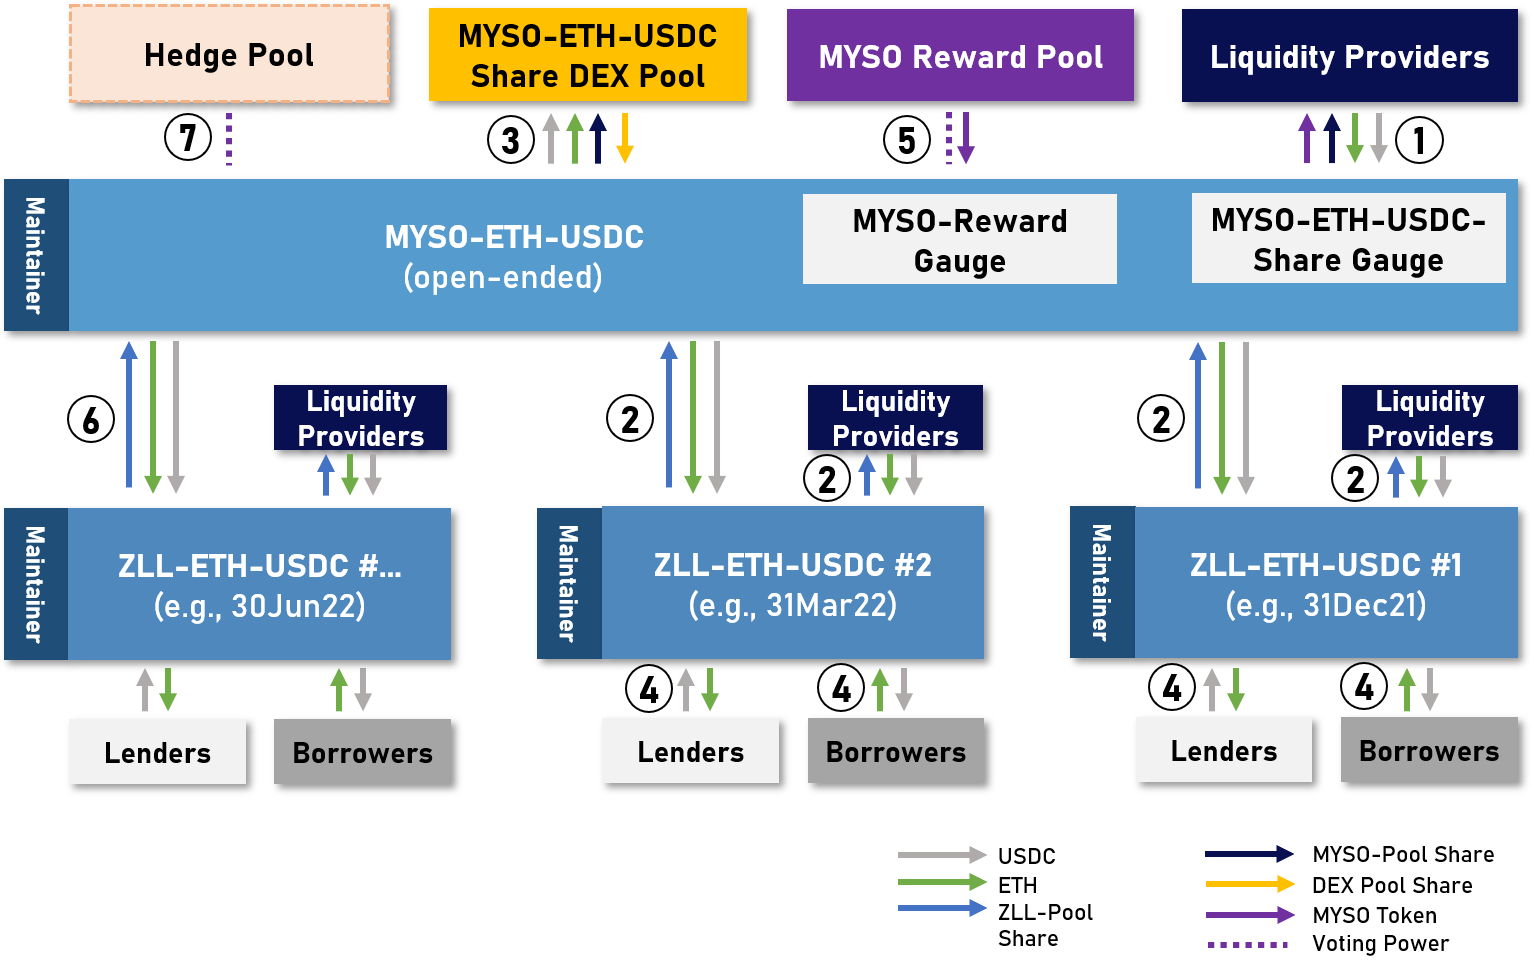
\includegraphics[width=1.0\textwidth]{figures/meta-pool.png} 
    \cprotect\caption{\small Overview of a ETH-USD denominated Meta-Pool with corresponding zero-liquidation loan pools. The labeled and enumerated interaction points are described in \cref{sec:walkthrough}.}
    \label{fig:meta-pool}
\end{figure}


\subsubsection{Roles \& Components}
\label{sec:roles}
As illustrated in \cref{fig:meta-pool}, the overall \emph{Meta-Pool} ecosystem is comprised of the following roles and components:
\begin{itemize}
    \item \textbf{Borrower}: pledges collateral to, and borrows funds from a zero-liquidation loan pool, which gives him an option to reclaim his collateral for a pre-agreed repayment amount after expiry.
    \item \textbf{Lender}: lends funds to a zero-liquidation loan pool, where the lent amount is secured by collateral posted by the pool. The lender either receives a pre-defined repayment amount (in case the loan pool's \emph{maintainer} exercises the pool's option), or otherwise the previously pledged collateral.
    \item \textbf{Zero-liquidation loan pool}: a liquidity pool that facilitates borrowing and lending using an AMM. During an initial subscription phase, liquidity providers can provide capital, which then becomes locked until expiry of the market. After expiry, liquidity providers can redeem their shares for a pro-rata share of the final funds held in the pool. For more details on the different pool phases as well as the AMM, please refer to \cite{sardon}.
    \item \textbf{Maintainer (of single pool)}: maintains a zero-liquidation pool, i.e., responsible for initializing a market, setting pricing parameters and triggering repayments towards lenders, where economically sensible.
    \item \textbf{Liquidity provider (of single pool)}: provides liquidity to a zero-liquidation loan pool and in return receives corresponding shares. At expiry of the pool, liquidity providers can redeem their shares with the given pool. 
    \item \textbf{Meta-pool}: a pool that provides liquidity to several zero-liquidation loan pools on an ongoing basis. All of the initially provisioned funds are subject to a lock-up period, but thereafter become redeemable at all times for a pro-rata share of all of the pool's holdings. In contrast to an individual zero-liquidation loan pool, the \emph{Meta-Pool} is open-ended. The \emph{Meta-Pool} can expand its TVL by minting new pool shares and selling them to liquidity providers. This process is regulated by a \emph{share gauge}, which is governed by MYSO token holders.
    \item \textbf{Meta-pool share gauge}: regulates the quantity of new shares to be minted as well as the price at which they shall be offered to liquidity providers. The gauge is governed by MYSO token holders.
    \item \textbf{MYSO-reward gauge}: analogous to Curve's gauge \cite{curve}, i.e., defines the quantity of rewards to be received by the given pool. The reward gauge is configured by MYSO token holders.
    \item \textbf{Maintainer (of meta-pool)}: maintains a \emph{Meta-Pool}, i.e., responsible for selecting suitable zero-liquidation pools and rolling over investments from expired pools.
    \item \textbf{Liquidity provider (of meta-pool)}: provides liquidity to a \emph{Meta-Pool}, where it is utilized for (i) liquidity provisioning to individual zero-liquidation loan pools as well as for (ii) bootstraping a DEX-based secondary market for \emph{Meta-Pool} shares.
    \item \textbf{MYSO reward pool}: a reward pool from where MYSO tokens are distributed across the MYSO ecosystem according to a \emph{MYSO-Reward Gauge}.
    \item \textbf{MYSO token}: a governance token which gives its holder voting power to adjust \emph{Meta-Pool} share gauges, MYSO reward gauges and give hedging mandates.
    \item \textbf{DEX for meta-pool shares}: a DEX-based market, where \emph{Meta-Pool} shares can be traded for the relevant currencies (e.g., \verb|ETH| and \verb|USDC|). 
    \item \textbf{Hedge Pool}: a pool that offers a hedge portfolio for the \emph{Meta-Pool's} overall risk position. For example, a hedge portfolio may be constructed by using \verb|ETH/USDC| perpetuals that make the \emph{Meta-Pool's} overall position (approximately) delta-neutral. MYSO token holders have voting power to give corresponding hedging mandates.
\end{itemize}

\subsubsection{Walkthrough of Common Interactions}
\label{sec:walkthrough}
The most common interaction points among the different parties and components of a \emph{Meta-Pool} ecosystem are enumerated in \cref{fig:meta-pool}, and explained in the following:
\begin{enumerate}
    \item Shown at the top of \cref{fig:meta-pool}, liquidity providers of the \emph{Meta-Pool} \verb|MYSO-ETH-USDC| provide \verb|ETH| and \verb|USDC| and in return receive \verb|MYSO-ETH-USDC-Shares|.
    \item Once sufficient liquidity has been amassed in the \verb|MYSO-ETH-USDC| \emph{Meta-Pool}, a maintainer then deploys capital to the zero-liquidation loan pools \verb|ZLL-ETH-USDC #1| and  \verb|ZLL-ETH-USDC #2|. In return the \emph{Meta-Pool} now holds shares in both of these pools. In addition, liquidity providers may also individually provide liquidity on a single zero-liquidation loan pool basis.
    \item Part of the \emph{Meta-Pool's} initial funds as well as the initial share supply are allocated to a DEX-based pool. In return, the \emph{Meta-Pool} receives shares in the DEX pool and thereby earns secondary market trading fees. 
    \item Borrower and lenders interact with each of the individual zero-liquidation loan pools.
    \item The \emph{Meta-Pool} receives MYSO token rewards, which are determined based on the pool's MYSO reward gauge.
    \item Once new suitable zero-liquidation loan pools become available, the maintainer rolls over funds.
    \item In the future, a \emph{Meta-Pool's} overall risk may be offset by using a hedge pool. For example, using a third-party protocol (e.g., perp.fi) one could construct a portfolio of perpetuals that provides an (approximate) delta hedge of the \emph{Meta-Pool's} total portfolio position. MYSO token holders can vote on whom to give a corresponding hedging mandate. 
\end{enumerate}

%\begin{center}
%    ...FURTHER WORK IN PROGRESS...
%\end{center}


\subsection{Meta-Pool Portfolio}
\label{sec:meta-pool-portfolio}
A \emph{Meta-Pool's} balance or holdings is comprised of the following currencies and pool shares:
\begin{itemize}
    \item \textbf{Collateral currency}: the collateral currency of the zero-liquidation loan pools to which liquidity shall be provided, e.g., \verb|ETH|. The respective quantity held by the \emph{Meta-Pool} is denoted by $\mathcal{Q}_{\mathcal{C}, t}$.
    \item \textbf{Borrow currency}: the borrow currency of the zero-liquidation loan pools to which liquidity shall be provided, e.g., \verb|USDC|. The corresponding quantity held by the \emph{Meta-Pool} is denoted by $\mathcal{Q}_{\mathcal{B}, t}$.
    \item \textbf{Zero-liquidation pool shares}: shares of the respective zero-liquidation pools to which liquidity has been provided, where the \emph{Meta-Pool's} held quantity is denoted by $\mathcal{Q}_{ZLL, j, t}$, and each pool is identified by an index $i=0,...,m$.
    \item \textbf{Meta-pool shares}: shares of the \emph{Meta-Pool}, where the quantity held by the \emph{Meta-Pool} is denoted by $\mathcal{Q}_{Meta, t}$.
    \item \textbf{DEX-pool shares}: shares in a DEX-based pool for \emph{Meta-Pool} shares, where the quantity held by the \emph{Meta-Pool} is denoted by $\mathcal{Q}_{DEX, i, t}$, and each pool is identified by an index $j=0,...,n$.
\end{itemize}

Initially, for each borrow currency unit the \emph{Meta-Pool} receives from liquidity providers an equal number of shares shall be issued. This means that at first the total number of shares is equal to the total received borrow currency amount, i.e., $\mathcal{Q}_{Meta, t=0} := \mathcal{Q}_{USDC, t=0}$. Note, however, that additional shares shall be issued in order to bootstrap the DEX-based secondary market. \cref{sec:meta-pool-shares} describes how this can be done without causing any unfair dilution for liquidity providers.\\

\subsubsection{Meta-Pool Shares Provided to DEX}
\label{sec:meta-pool-shares}
During the initial bootstrapping, the \emph{Meta-Pool} uses a fraction $0<f_{DEX}<1$ of its liquidity (i.e., $f_{DEX} \cdot \mathcal{Q}_{ETH, t=0}$, and $f_{DEX} \cdot \mathcal{Q}_{USDC, t=0}$) to kick-start a secondary market for its shares. Note that for a liquidity provider $k$ who provides $\mathcal{Q}_{USDC, k, t=0}$ and $\mathcal{Q}_{ETH, k, t=0}$ in liquidity, his directly held relative share in the \emph{Meta-Pool} will be smaller than $\frac{\mathcal{Q}_{USDC, k, t=0}}{\sum_k \mathcal{Q}_{USDC, k, t=0}}$. This is because after issuing shares to the initial liquidity providers, the pool will mint additional shares, which it will use as inventory for its DEX-based share pool market. However, this doesn't cause any dilution for liquidity providers because when they redeem shares, in addition to receiving \verb|ETH| and \verb|USDC|, they also receive back pool shares\footnote{More specifically, they receive back DEX-based LP shares that are redeemable for \emph{Meta-Pool} shares.}, which allow them to again redeem funds and pool shares, which again are redeemable for funds and pool shares, and so on. This ``recursive redemption'' can be expressed as a geometric series, i.e.,
\begin{equation}
\begin{split}
\label{eq:meta-pool-share}
V_{\mathcal{U}} &= s_{\mathcal{U}} \Bigg( V_{\mathcal{P}} + s_{\mathcal{P}} \bigg( V_{\mathcal{P}} + s_{\mathcal{P}} \Big(  V_{\mathcal{P}} + s_{\mathcal{P}} \big( ... \big) \Big) \bigg) \Bigg)\\
 &= \frac{s_{\mathcal{U}} V_{\mathcal{P}}}{1 - s_{\mathcal{P}}}
\end{split}
\end{equation}
where $s_{\mathcal{U}}$ is the liquidity provider's share in the pool, $s_{\mathcal{P}}:=f_{DEX}$ is the fraction of pool shares held by the pool itself, $V_{\mathcal{P}}$ is the value held by the pool (i.e., total value of \verb|ETH| and \verb|USDC| holdings), and $V_{\mathcal{U}}$ denotes the value of the liquidity provider's position in the \emph{Meta-Pool} (i.e., total value of \verb|ETH| and \verb|USDC| holdings).\\

For example, assume there's a liquidity provider that has contributed $V_{\mathcal{U}}=100'000$ in combined \verb|ETH| and \verb|USDC| liquidity to a \emph{Meta-Pool}, and assume the value of total accumulated liquidity in the pool is $V_{\mathcal{P}}=1'000'000$. Assuming there's an initial DEX allocation of $s_{\mathcal{P}}=f_{DEX}=10\%$, one can then use \cref{eq:meta-pool-share} to calculate the liquidity provider's ``target share'', i.e.,
\begin{equation}
\begin{split}
s_{\mathcal{U}} &= \frac{V_{\mathcal{U}}(1-s_{\mathcal{P}})}{V_{\mathcal{P}}}.
\end{split}
\end{equation}
Hence, the liquidity provider's resulting relative share is $s_{\mathcal{U}} = \frac{100'000}{1'000'000} \cdot (1-10\%)=9\%$. An alternative obvious way to express his relative share is as the ratio between the number of shares held by the liquidity provider and the overall supply, i.e.,
\begin{equation}
\begin{split}
s_{\mathcal{U}} &= \frac{N_{\mathcal{U}}}{N_{\mathcal{U}} + N_{\mathcal{P}} + N_{other}}.
\end{split}
\end{equation}
Based on this one can can then derive $N_\mathcal{P}$, i.e., the amount of additionally to be minted shares. For example, if the absolute share quantity held by the liquidity provider is $N_{\mathcal{U}}=80'000$ (e.g., assuming he provided $\mathcal{Q}_{USDC, k, t=0}=80'000$), and the quantity held by others is $N_{other}=720'000$, then the required quantity of pool shares $N_{\mathcal{P}}$ to be issued and provided to the DEX can be calculated using
\begin{equation}
\begin{split}
N_{\mathcal{P}} &= N_{\mathcal{U}} \Bigg( \frac{1}{s_{\mathcal{U}}} - 1 \Bigg) - N_{other}
\end{split}
\end{equation}
, which leads to $N_{\mathcal{P}}=80'000\cdot (1/9\% - 1) - 720'000=88'888.89$. \cref{tab:meta-pool-shares} shows how an iterative redemption by the liquidity provider allows him to effectively reclaim his originally pledged value, i.e., the sum of the recursively redeemed values in column $V_{\mathcal{U}}$ converges to the initially pledged value of $100'000$.

\begin{table}
\captionsetup{font=scriptsize}
\scriptsize	
% created with https://www.latex-tables.com/#
\centering
\begin{tabular}{rrrrrrr}
\textbf{\#} & $N_{\mathcal{U}}$ & $V_{\mathcal{U}}$ & $V_{\mathcal{P}}$ & $N_{\mathcal{P}}$ & $N_{other}$ & $N_{\mathcal{U}} + N_{\mathcal{P}} + N_{other}$ \\ 
\hline
1                                & 80,000.00                                & -                                         & 1,000,000.00                                   & 88,888.89                                & 720,000.00                                 & 888,888.89                          \\
2                                & 8,000.00                                 & 90,000.00                                 & 910,000.00                                     & 80,888.89                                & 720,000.00                                 & 808,888.89                          \\
3                                & 800.00                                   & 9,000.00                                  & 901,000.00                                     & 80,088.89                                & 720,000.00                                 & 800,888.89                          \\
4                                & 80.00                                    & 900.00                                    & 900,100.00                                     & 80,008.89                                & 720,000.00                                 & 800,088.89                          \\
5                                & 8.00                                     & 90.00                                     & 900,010.00                                     & 80,000.89                                & 720,000.00                                 & 800,008.89                          \\
6                                & 0.80                                     & 9.00                                      & 900,001.00                                     & 80,000.09                                & 720,000.00                                 & 800,000.89                          \\
7                                & 0.08                                     & 0.90                                      & 900,000.10                                     & 80,000.01                                & 720,000.00                                 & 800,000.09                          \\
8                                & 0.01                                     & 0.09                                      & 900,000.01                                     & 80,000.00                                & 720,000.00                                 & 800,000.01                          \\
9                                & 0.00                                     & 0.01                                      & 900,000.00                                     & 80,000.00                                & 720,000.00                                 & 800,000.00                         
\end{tabular}
\caption{\label{tab:meta-pool-shares}Example of a liquidity provider iteratively redeeming his pool shares for funds and pool shares, and so on. Note that the total iteratively redeemed value $V_{\mathcal{U}}$ converges to the originally provided value $100'000$, as expected.}
\end{table}

%Let $\mathcal{Q}_{ETH, t}$ and $\mathcal{Q}_{USDC, t}$ denote the amount of liquidity provided to the \emph{Meta-Pool} at time $t$. The quantity of initially issued \emph{Meta-Pool} shares shall be denoted by $\mathcal{Q}_{Meta, t}$, where $\mathcal{Q}_{Meta, t=0} := \mathcal{Q}_{USDC, t=0}$, i.e., initially for each unit of borrow currency an equal amount of shares is issued. Initially, the \emph{Meta-Pool} will provide a fraction $0<c_{DEX}<1$ of liquidity into a DEX pool and reserve the remainder $1-c_{DEX}$ as funding for zero-liquidation loan pools. The quantity of DEX share pools shall be denoted by $\mathcal{Q}_{DEX, t, i}$, and the quantity of zero-liquidation loan pool shares by $\mathcal{Q}_{ZLL, t, j}$, where each DEX pool is indexed by $j=0,...,n$ and each zero-liquidation loan pool by $j=0,...,m$.\\

\subsubsection{DEX-Pool Liquidity}
\label{sec:dex}
As described in \cref{sec:meta-pool-shares}, each \emph{Meta-Pool} reserves a certain amount of \emph{Meta-Pool} shares and borrow/collateral currency (e.g., \verb|ETH| and \verb|USDC|) to kick-start its own DEX pool. Naturally, balancer is a good choice for such a DEX pool because it allows dealing with more than two currencies (i.e., here pool shares, \verb|ETH| and \verb|USDC|). In return for providing liquidity to the DEX pool, the \emph{Meta-Pool} receives corresponding LP shares, which lets it earn trading fees from secondary market activity. Note that ``new'' liquidity providers can also directly add liquidity to such a DEX pool. However, in case they haven't participated in the initial bootstrapping phase or acquired shares through subsequent new issuances would need to use \emph{single-asset-deposits}, which will cost swap fees and cause \emph{Meta-Pool} shares to appreciate in value \cite{balancer}. 

\subsection{Liquidity Providing Risks}
\label{sec:hedging}
The risk of providing liquidity to a \emph{Meta-Pool} is predominantly the aggregate risk of providing liquidity to several zero-liquidation loan pools with different expiry dates.\footnote{Note that \emph{Meta-Pool} shareholders are also exposed to the market making risk associated with providing liquidity to the DEX-based pool for pool shares.} Recall that a liquidity provider in a zero-liquidation loan pool is essentially selling covered calls to borrowers, and buying call options from lenders \cite{sardon}. The corresponding PnL and risk profile is illustrated in \cref{fig:lp-risk-1} and \cref{fig:lp-risk-2}, where one can see that, naturally, a liquidity provider is synthetically long the given underlying asset (e.g., \verb|ETH/USDC|).\\

%As with any liquidity pool, liquidity providers of \emph{Meta-Pools} are exposed to the risk of trading against informed order flow and inventory risk. Moreover, and more specifically to options market making, liquidity providers of zero-liquidation loan pools (and hence also of \emph{Meta-Pools}) bear the typical risk of being unable to continuously rebalance and hedge the pool's overall option portfolio \cite{jameson}.

\begin{figure}
    \centering
    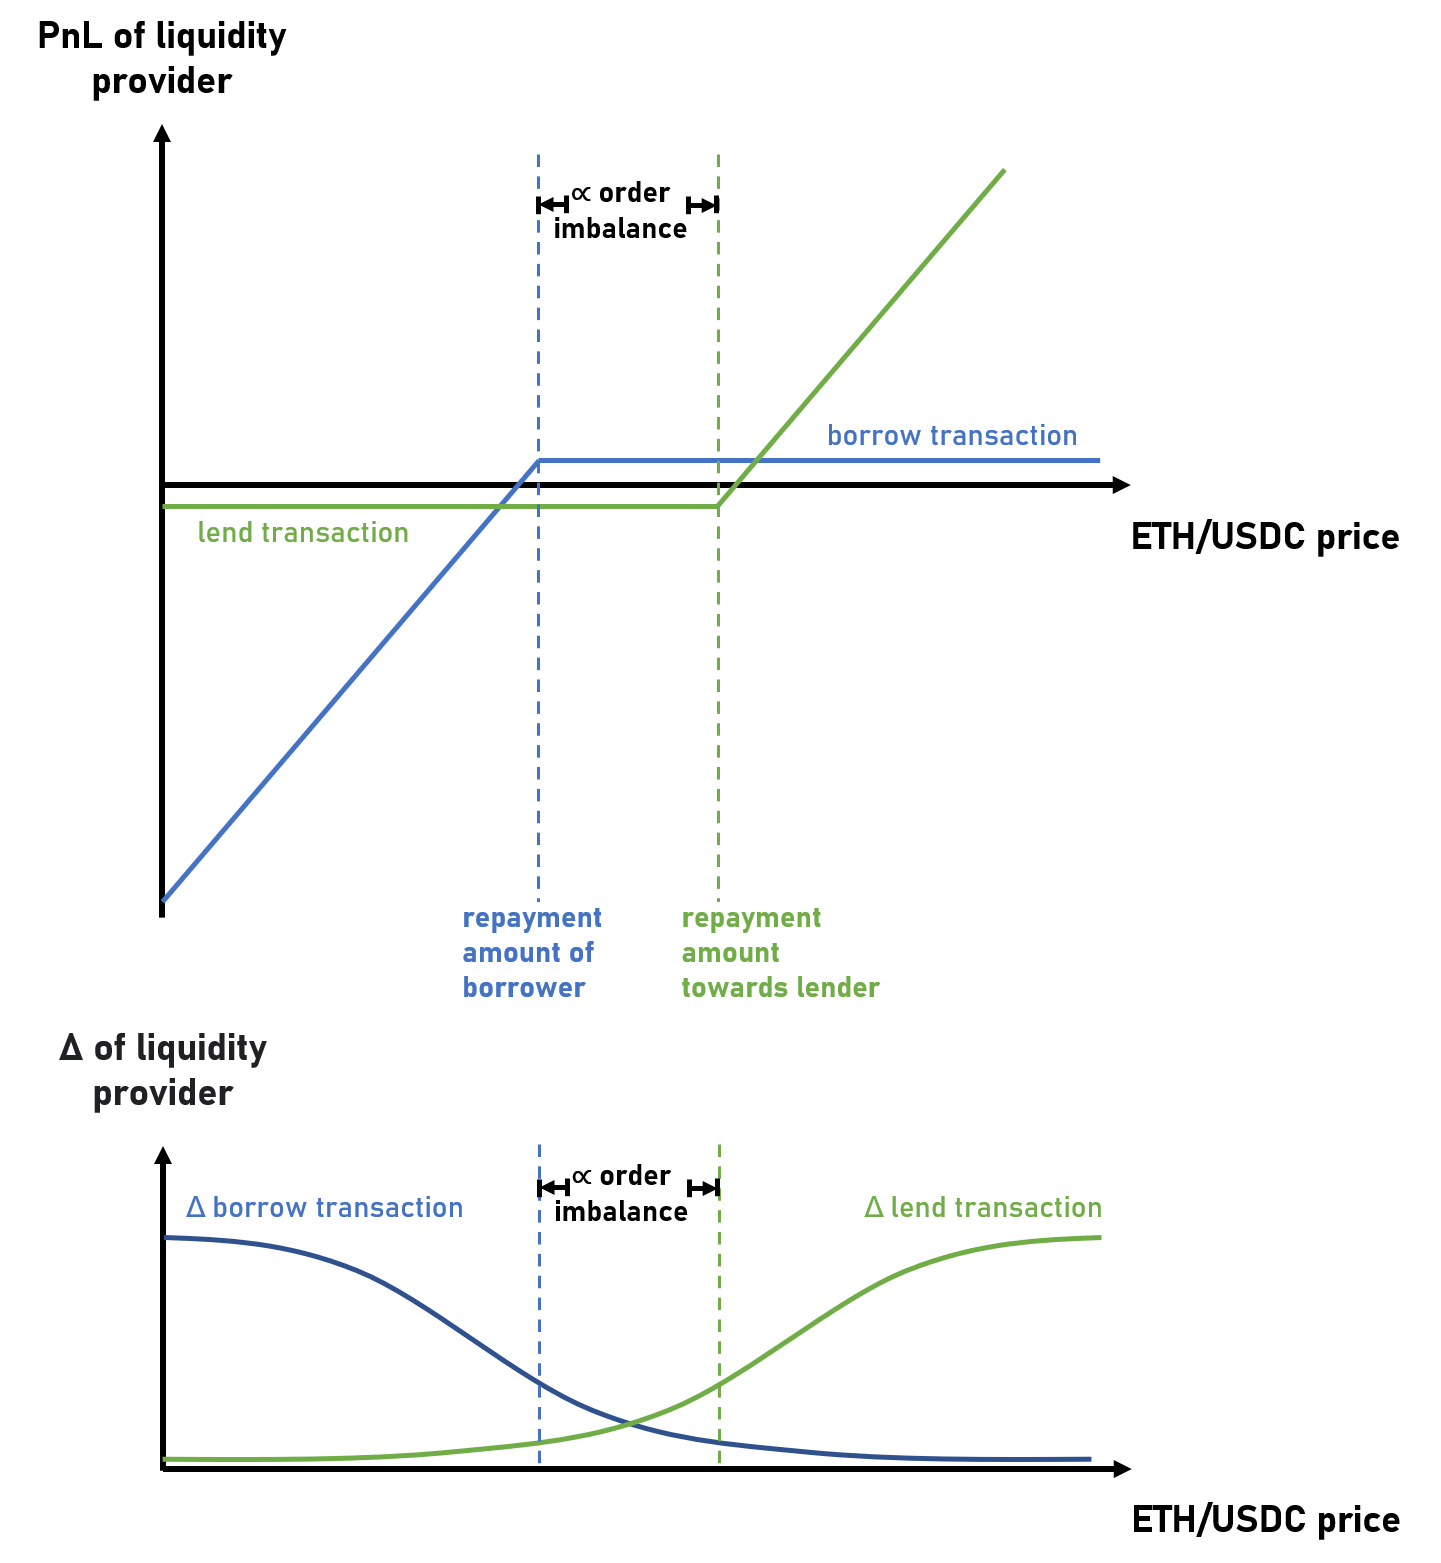
\includegraphics[width=0.78\textwidth]{figures/lp-risk-1.png} 
    \cprotect\caption{\small Illustration of a liquidity provider's PnL and associated $\Delta$ risk profile for a zero-liquidation loan pool.}
    \label{fig:lp-risk-1}
\end{figure}

The risks of the liquidity provider's overall option position can be described by the corresponding option sensitivities or \emph{greeks}. The bottom of \cref{fig:lp-risk-1} and \cref{fig:lp-risk-2} illustrates the stylized delta risk profile, i.e., the changes in portfolio value resulting from changes in the underlying price. Note that the \emph{Meta-Pool's} overall delta is the sum of the delta of all zero-liquidation loan pool's, which in turn is simply the sum of the weighted individual option deltas \cite{frei}, i.e.,

\begin{equation}
\begin{split}
\label{eq:delta-risk}
\small
\Delta_{Meta} &= \frac{\partial \Pi_{Meta}}{\partial S} \\
& = \sum_j \frac{\partial \Pi_{ZLL, j}}{\partial S} \\
& = \underbrace{\sum_{b \in \mathcal{B}} w(b) \Big( 1 - \frac{\partial C_{K(b), T(b)}}{\partial S} \Big) }_{\textrm{=from borrows}} + \underbrace{\sum_{l \in \mathcal{L}} w(l) \Big( \frac{\partial C_{K(l), T(l)}}{\partial S} \Big) }_{\textrm{=from lends}}
\end{split}
\end{equation}

, where $\Pi$ denotes the corresponding portfolio value, $S$ is the underlying price, $\mathcal{B}$ denotes the set of options associated with borrows, $\mathcal{L}$ the one associated with lends, $w(...)$ is the weight of the given option position, and $C_{K(...), T(...)}$ is the price of a call option with strike $K(...)$, and expiry date $T(...)$.\\

Naturally, the \emph{Meta-Pool's} delta-risk will depend on the degree of order flow imbalance in borrows and lends. Recall that the ``floating strike'' of a zero-liquidation loan's embedded option is pushed downwards through borrow transactions, and upwards through lends \cite{sardon}. In case there's well balanced order flow between borrows and lends, then the resulting ``weighted distance''\footnote{Weighted with regards to the given zero-liquidation loan's size.} between the strikes of sold covered calls, and bought calls will be rather small as the upward and downward pushes offset each other. It is easy to see that in case both strikes are very close to one another, the resulting PnL and risk profile is approximately the same as holding the underlying because: $\lim_{K'\to K} (Covered \; Call \; C_{K}) + C_{K'}=\lim_{K\to K'}(S - C_{K})+C_{K'}=S$. From a hedging perspective this means that the need to dynamically rehedge delta is reduced in these instances because the delta sensitivity itself becomes lower, i.e., $\Gamma = \frac{\partial S}{\partial S^2} \to 0$, enabling simple static hedging. In contrast, the more imbalanced the order flow is, the greater the distance between the strikes becomes, thus making the risk profile less ``delta-1'' like, and hence making hedging more cumbersome as rehedging has to be done more frequently. 

\subsubsection{Hedge Pool}
The delta risk of the portfolio (see \cref{eq:delta-risk}) can be hedged by shorting the corresponding quantity $\Delta_{Meta}$ of underlyings. For example, one can construct a portfolio of perpetuals that (approximately) offsets the \emph{Meta-Pool's} delta risk. Naturally, there could be different ways how to exactly structure such a portfolio (e.g., using perpetuals from dYdX or Perpetual Protocol, or options from opyn). \emph{Meta-Pools} don't dictate how such a portfolio or \emph{hedge pool} should look like, but leave it to the market to decide. More specifically, MYSO token holders can vote which hedge pool they view as the ``best'' hedge solution for a given \emph{Meta-Pool}. This means they have decision power about if and how the TVL of a \emph{Meta-Pool} shall be hedged, and, ultimately, whom to give a ``hedge mandate''.\\

Naturally, the process of creating and maintaining a hedge pool involves work. For example, in order to maintain an overall delta-neutral position one needs to continuously rebalance the delta hedge. Note, however, that hedging on an aggregate portfolio basis of a \emph{Meta-Pool} instead of individually is beneficial for the MYSO ecosystem because it allows for greater economies of scale, e.g., with regards to transaction costs or lower hedging frequency requirements \cite{peeters}. In addition, hedging on an aggregate level also leads to a larger TVL size of a corresponding hedge mandate, thus making it more attractive for third parties to develop hedge solutions as they can potentially steer significant order sizes and corresponding transaction fees.\\

Hedge pool providers can be compensated with MYSO tokens for their work. An example of how such a hedge pool transaction could be structured and carried out is illustrated in \cref{fig:hedge-pool}. Here, \emph{Meta-Pool} holders pledge their pool shares into a hedge pool, for which they then receive corresponding hedge pool shares, which are redeemable for a pro-rata share of the overall funds held in the hedge pool. Ideally, and in order to maximize capital efficiency, the \emph{Meta-Pool} shares would be recognized as collateral with a third party protocol from where the corresponding hedge instruments (e.g., perpetuals) are bought. Alternatively (or additionally), the hedge provider may fund or pool collateral himself, and in return own part of the hedge pool shares, in order to ensure he also has ``skin in the game''. The hedge provider could then initiate and maintain a corresponding hedge portfolio, and MYSO token holders could delegate rewards to him by setting the \emph{Meta-Pool's} MYSO reward gauge accordingly.
\begin{figure}
    \centering
    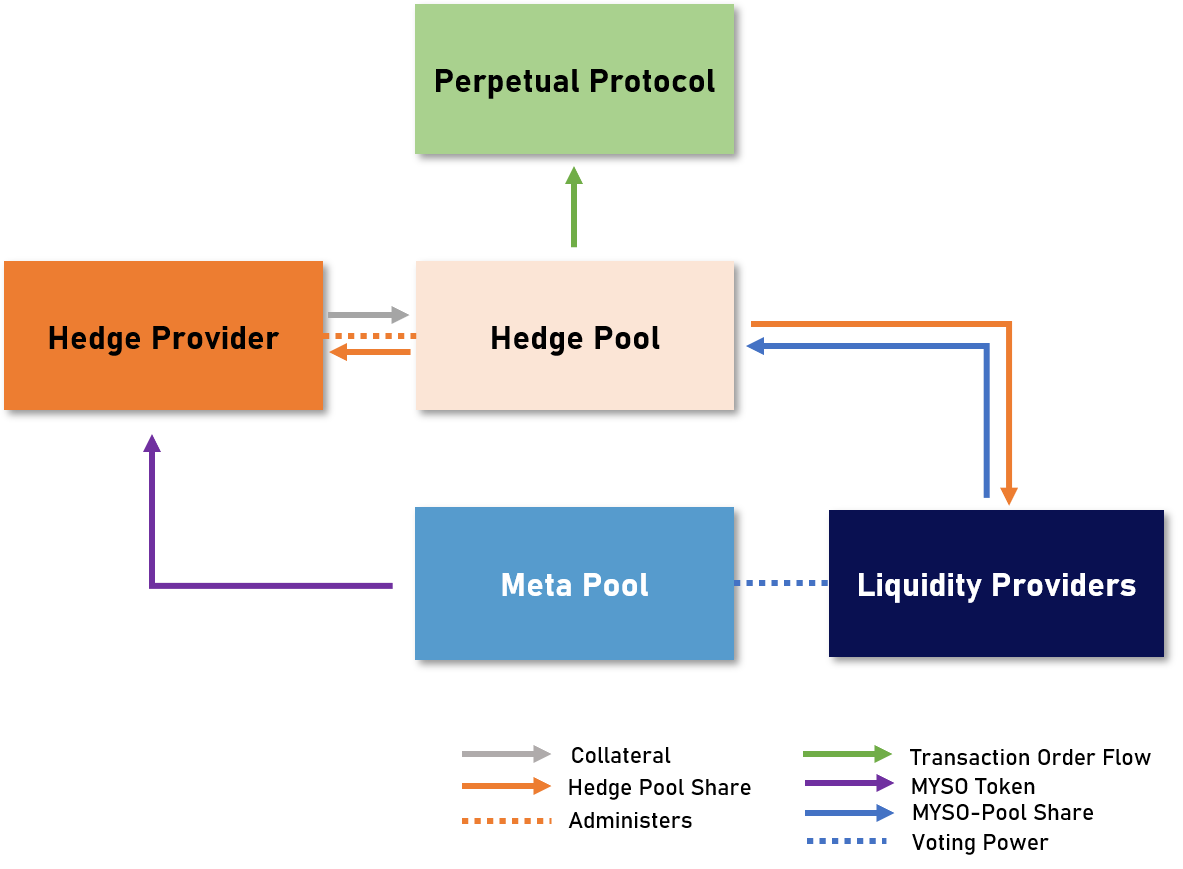
\includegraphics[width=0.88\textwidth]{figures/hedge-pool.png} 
    \cprotect\caption{\small Example of how a hedge pool mandate could be structured and carried out.}
    \label{fig:hedge-pool}
\end{figure}


\section{Governance}
\label{sec:governance}
\emph{Meta-Pools} shall be governed by MYSO token holders, who decide on (i) MYSO reward gauge settings, (ii) rewards for hedge pool providers and (iii) gauge settings for \emph{Meta-Pool} share issuances. In addition, MYSO token holders also have decision power over a treasury, and can create and vote over protocol proposals and changes.

\subsection{MYSO Token}
MYSO tokens are \emph{governance tokens} that distribute voting power across users and stakeholders (see \cref{sec:roles}) of the MYSO ecosystem. The purpose of the MYSO token is to foster community-driven decision making and collaboration, both within the MYSO community as well as with the wider DeFi ecosystem. Note that analogous to YFI tokens, MYSO tokens are \emph{valueless} \cite{yearn}, and don't represent any cash flow rights.

\subsubsection{Initial Distribution}
The initial MYSO token supply will be $100'000'000$ MYSO and shall be distributed across pre-launch investors, core team, advisors, test users, airdrops, liquidity rewards and a treasury as follows:
\begin{itemize}
    \item \textbf{Pre-launch investors}: $8'000'000$ (8.0\%)
    \item \textbf{Team}: $18'000'000$ (18.0\%)
    \item \textbf{Advisors}: $2'000'000$ (2.0\%)
    \item \textbf{Incentivized testnet}: $500'000$ (0.5\%)
    \item \textbf{Airdrops}: $500'000$ (0.5\%)
    \item \textbf{Liquidity rewards}: $22'500'000$ (22.5\%)
    \item \textbf{Treasury}: $48'500'000$ (48.5\%)
\end{itemize}
The distribution is based on a 3:1 split between ``outsiders'' and ``insiders'' as advocated by Placeholder \cite{placeholder}, i.e., the majority of tokens (72.0\%) is reserved for the community, whereas a smaller remainder (28.0\%) is allocated to pre-launch investors, core team and advisors. \cref{fig:token-split} shows how the MYSO token split compares to other DeFi projects, from which one can see that the MYSO token distribution is set in favor of a higher community allocation.

\begin{figure}
    \centering
    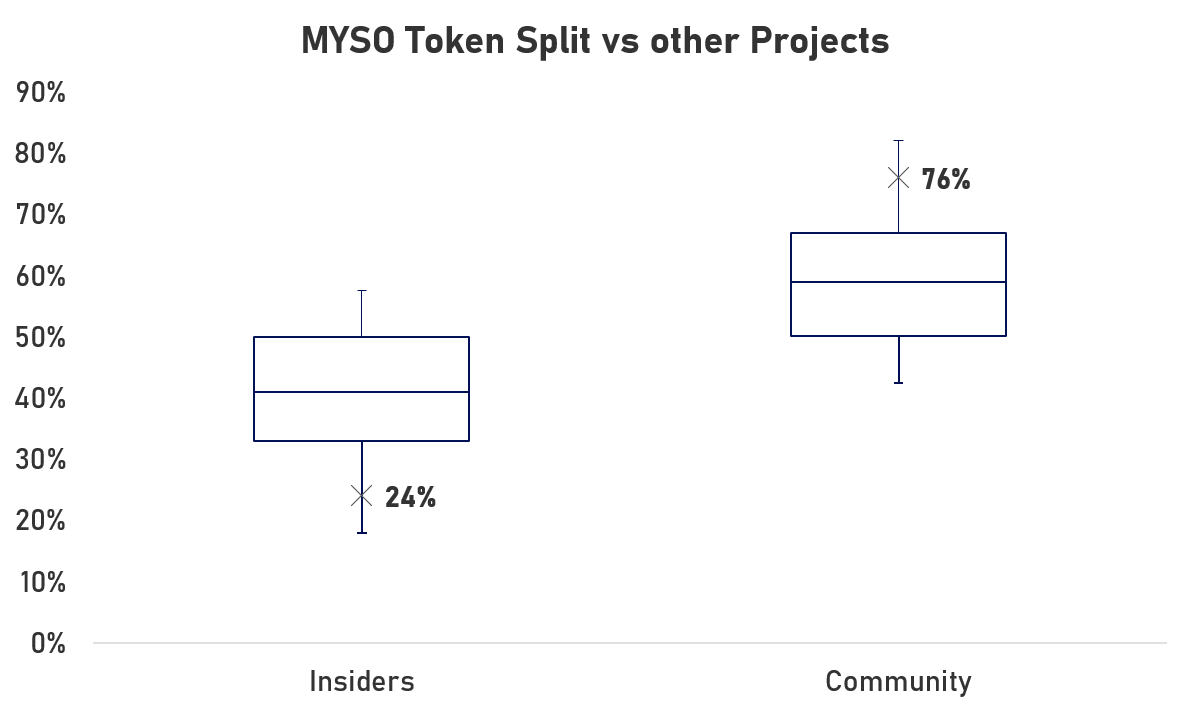
\includegraphics[width=0.88\textwidth]{figures/token-split.png} 
    \cprotect\caption{\small Boxplot comparing the MYSO token split with other DeFi projects, i.e., Uniswap, Futureswap, Radicle, Balancer, Fei, UMA, Curve, FRAX, Reflexer, Liquity, Compound, Aave, InstaDapp \cite{gyroscope}.}
    \label{fig:token-split}
\end{figure}

\subsubsection{Treasury}
A significant share of the initial MYSO token supply (48.5\%) will be allocated to a smart contract treasury, which shall be governed by the MYSO token holders. The purpose of the treasury is to support the long-term development of the MYSO ecosystem, foster innovation (e.g., providing grants for third-party integrations), and accelerate growth (e.g., funding new product developments or sponsoring additional liquidity mining programs).

\subsubsection{Gauges}
As shown in \cref{fig:meta-pool}, each \emph{Meta-Pool} has two gauges, i.e., (i) a MYSO rewards gauge that controls how many MYSO rewards shall be made available for distribution to share holders of a given pool, and (ii) a pool share gauge that regulates how many new shares shall be offered to liquidity providers and for which price. 

\subsubsection{Liquidity Rewards}
Users can earn MYSO tokens by providing liquidity to \emph{Meta-Pools} and staking the pool share tokens in a MYSO reward smart contracts, from which they can then claim their MYSO token rewards. The reward amount and frequency is controlled by MYSO token holders. At launch there will be one ``genesis'' \emph{Meta-Pool}, which shall be eligible to distribute $2'800'000$ MYSO token rewards over a period of 1 month. Note that the liquidity rewards program is subject to changes and might be revised in order to adapt to user behavior and market dynamics.\footnote{Generally speaking, the liquidity rewards program shall attract early and long-term oriented liquidity. Moreover, the overall duration of the liquidity mining program shall be shortened as much as possible to create momentum, and rewards shall be subject to a vesting schedule to reduce the potential of pump-and-dumps. Lastly, the liquidity rewards shall also take advantage of opportunities in cross-product and cross-protocol community engagement (e.g., airdrops might be targeted at users that have suffered from liquidations in the past or shown ``positive'' liquidity provisioning behavior in similar protocols).} After the initial launch, MYSO token holders may vote on adding new \emph{Meta-Pools} as well as the corresponding reward allocation for each pool.

\subsubsection{Meta-Pool Shares}
Initially, a \emph{Meta-Pool's} share supply will be determined based on the initial liquidity contributions and DEX allocation (see \cref{sec:meta-pool-shares}). Thereafter, \emph{Meta-Pools} can additionally mint and offer pool shares to liquidity providers in order to expand their TVL base. The issuance amount and price is set by MYSO token holders, who can use the DEX-based secondary market dynamics and prices as guidance. For example, in order to stimulate growth in a certain \emph{Meta-Pool} MYSO token holders may decide to offer corresponding pool shares at a discount to market participants.

\newpage
\appendix
\section{Appendix}

\begin{figure}[!ht]
    \centering
    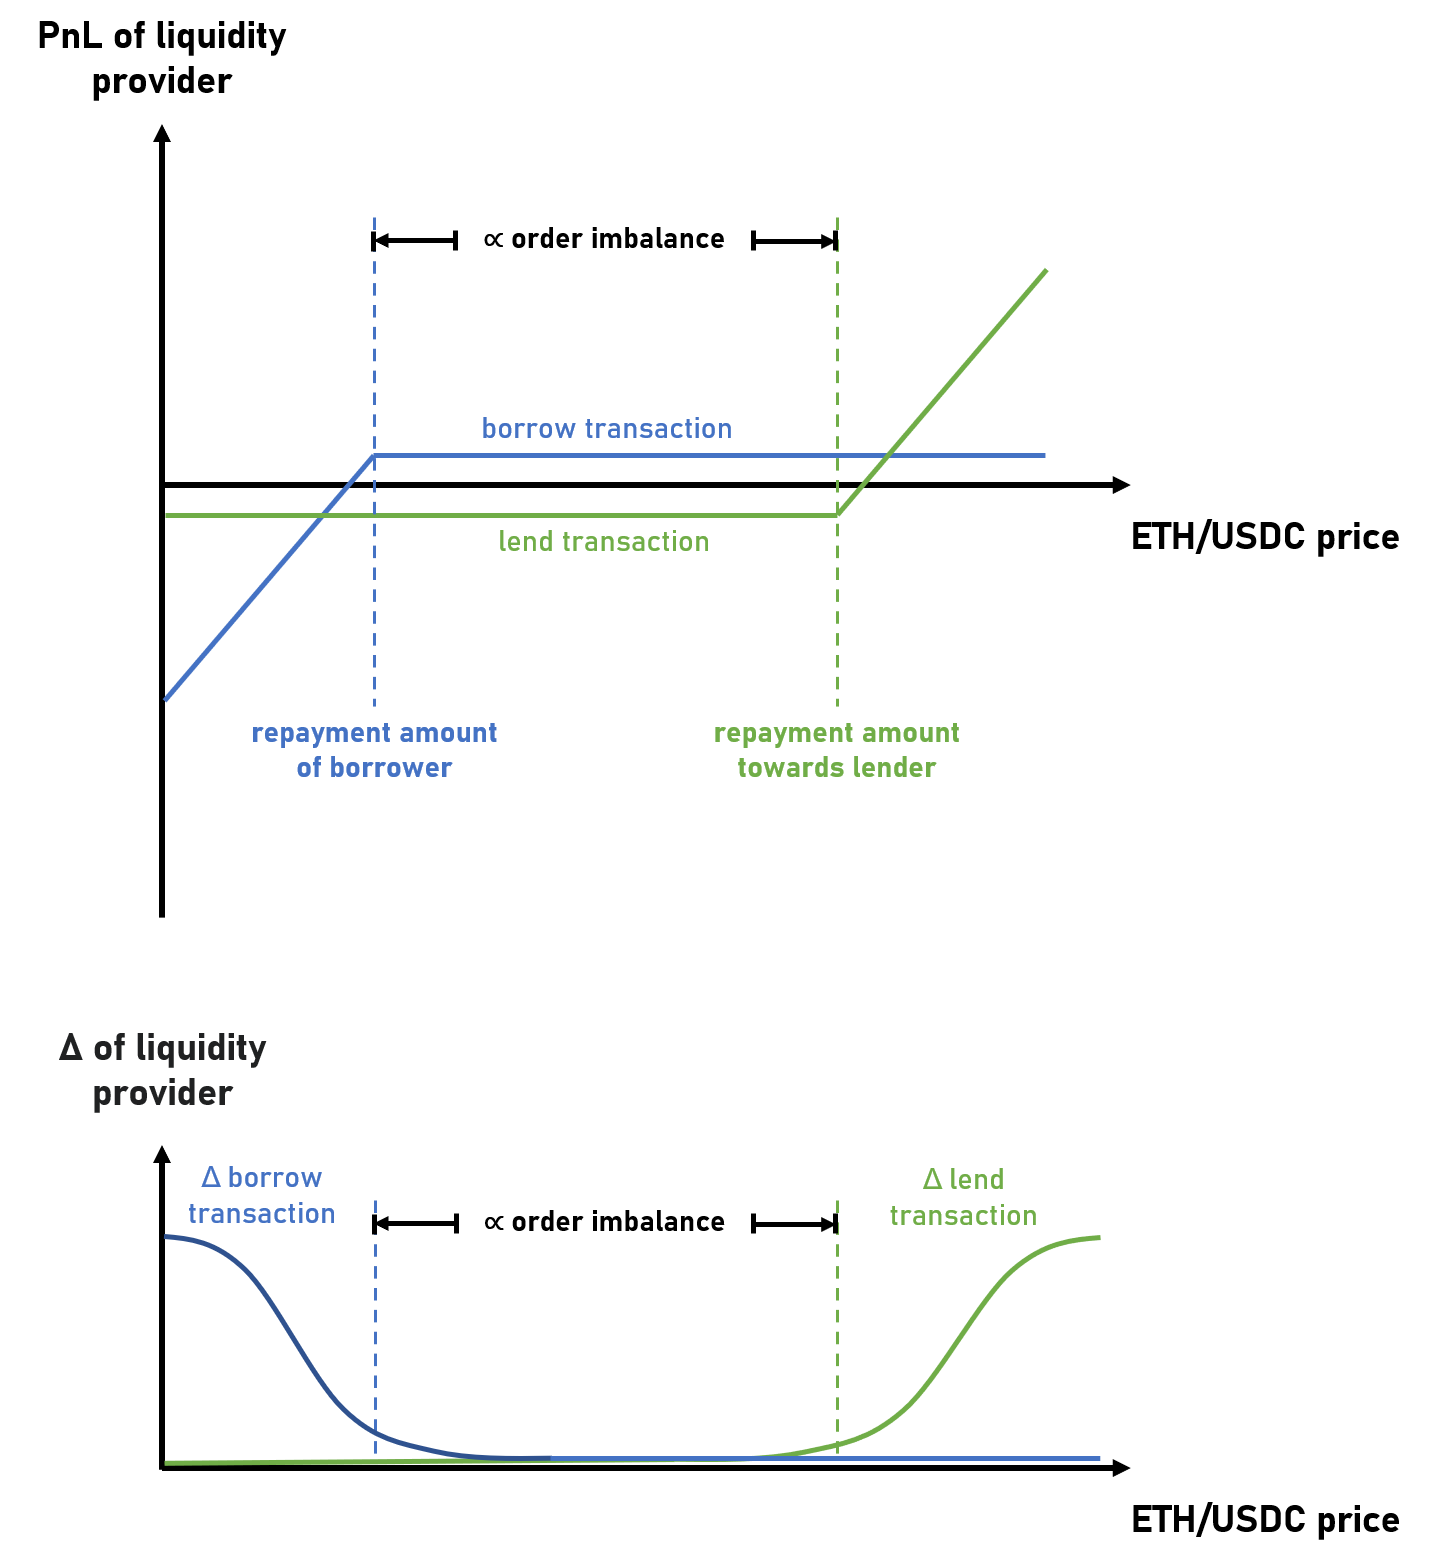
\includegraphics[width=0.78\textwidth]{figures/lp-risk-2.png} 
    \cprotect\caption{\small Same as \cref{fig:lp-risk-1} but with a more imbalanced order flow, leading to a higher distance between the strikes of sold covered calls and bought calls.}
    \label{fig:lp-risk-2}
\end{figure}

\newpage
\bibliographystyle{abbrv}
\bibliography{main}

\end{document}
